\begin{tframe}{Standard Training}

The net was trained in a standard way, using the 60,000 images of the train and validation sets. The training went on for 30 epochs.

\vspace{0.1in}

The tests carried out on the trained model were of two kind. 

\vspace{0.1in}

The first test was made using the 10,000 clean samples from the testing set; the second test was made using the adversarial examples, that is the same samples as the first test but with an added perturbation computed as shown previously.

\end{tframe}

\begin{tframe}{Standard Training}

\begin{center}
  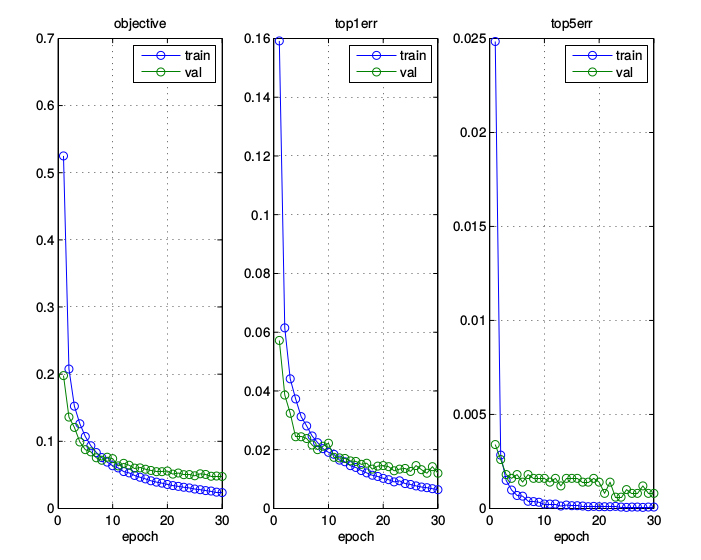
\includegraphics[width=0.7\textwidth]{img/train-base.png}
	\label{train-base} 
\end{center}
\end{tframe}

\begin{tframe}{Standard Training}

\begin{table}[h]
\centering
\begin{tabular}{@{}lll@{}}
\toprule
                               & Clean & Adversarial \\ \midrule
Correctly Predicted            & 98.47 & 3.36        \\
Error                          & 1.53  & 96.64       \\
Confidence                     & 98.59 & 93.82       \\
Confidence Correctly Predicted & 99.04 & 91.67       \\
Confidence Error               & 69.95 & 93.89       \\ \bottomrule
\end{tabular}
\end{table}

As we can see from the results, the classification using the clean samples as test images worked great, with high prediction rate and confidence. The results for the adversarial test, however, behaved as expected, with a large percentage of misclassification with a high confidence.

\end{tframe}